
%
%  $Description: Author guidelines and sample document in LaTeX 2.09$ 
%
%  $Author: ienne $
%  $Date: 1995/09/15 15:20:59 $
%  $Revision: 1.4 $
%

\documentclass[times, 10pt, twocolumn]{article} 
\usepackage{latex8}
\usepackage{times}
\usepackage{graphicx}
\usepackage{float}
\graphicspath{ {./images/} }
\usepackage{multicol}

%\documentstyle[times,art10,twocolumn,latex8]{article}

%------------------------------------------------------------------------- 
% take the % away on next line to produce the final camera-ready version 
\pagestyle{empty}

%------------------------------------------------------------------------- 
\begin{document}

\title{%
  \normalfont\large Instituto Superior Técnico — Taguspark \\
  \large Design and Implementation of Distributed Applications 2019-2020 \\
  \bigskip
  \bigskip
  \huge MSDAD \\
  \bigskip
  \medskip
  \Large Project Report — Group 19\\
}

\author{
David Gonçalves\\
ist173891
\and
André Moreira\\
ist187630\\
\and
Leonardo Troeira\\
ist194104\\
}

\maketitle
\thispagestyle{empty}

%------------------------------------------------------------------------- 
\Section{Introduction}
The goal of this project was to design, develop and evaluate a replicated distributed meeting scheduling system using a client-server model. A replicated set of servers provide services for reading the current open meeting proposals, creating and closing meetings, and joining meeting invitations. Meeting proposals once created are broadcast among system clients. The meeting scheduler is accessed via a remote client application on which users perform all schedule related operations as requests to the servers.

Our implementation includes all the functionality aforementioned. However, our diffusion algorithm, despite supporting N-1 faults (i.e. server crashes), has the downside of not scaling well, as a single server is responsible for informing all the other servers and clients when its state changes.

%-------------------------------------------------------------------------
\Section{Problem}
We are faced with several problems regarding distribution for implementing our meeting scheduling system. We have to assure the following properties:

\SubSection{Availability} 
Our system should have a balance between availability and scalability. It should tolerate a reasonable amount of faults while still being capable of responding to clients within an acceptable time frame.

\SubSection{Scalability}
As our system grows, i.e. number of servers and clients, it is important to distribute the load among the participants as to not compromise availability.

\SubSection{Synchronization}
It should not be possible for a meeting to be closed at the same time that someone is joining.

\SubSection{Fault tolerance}
Should a server crash, the system’s state and client’s usability should not be compromised. Our system should tolerate a number N of faults large enough to keep a balance between scalability and availability.

%------------------------------------------------------------------------- 
\Section{Achievements}

The list below presents the functionalities that we implemented in our solution:

\begin{itemize}
   \item PuppetMaster
   \begin{itemize}
     \item Launches Server(s) - Fully Implemented;
     \item Launches Client(s) - Fully Implemented;
     \item Freeze Server(s) - Fully Implemented;
     \item Unfreeze Server(s) - Fully Implemented;
     \item Crash Server(s) - Fully Implemented;
     \item Status - Fully Implemented;
     \item AddRoom(s) - Fully Implemented;
     \item Parser - Fully Implemented;
   \end{itemize}
   \item Client
   \begin{itemize}
     \item CreateMeeing(s) - Fully Implemented;
     \item JoinMeeting(s) - Fully Implemented;
     \item ListMeeting(s) - Fully Implemented;
     \item CloseMeetings(s) - Fully Implemented;
     \item Parser - Fully Implemented;
     \item Diffusion Algorithm - Server takes care of this;
   \end{itemize}
   \item Server
   \begin{itemize}
     \item Replication - Fully Implemented;
     \item Fault Tolerance - Fully Implemented;
     \item Message Delivery Delays - Fully Implemented;
     \item Diffusion Algorithm - Partially Implemented;
   \end{itemize}
\end{itemize}

\SubSection{PuppetMaster}

Our solution allows the Puppet Master to launch servers and clients (that will be created by the PCS), it also allows to manage servers with the following commands: Freeze; Unfreeze; Crash; AddRoom; Status.
Furthermore, the PuppetMaster can also execute a set of tasks from a script file.

\SubSection{Client}

In our solution the client is able to Create, Join, List and Close Meetings.
Our close meeting functionality chooses the date and location that maximizes the number of participants. Any attendees that cannot go to the meeting on that date and location are rejected. If there is no room capacity for all attendees, some are randomly rejected. Our client application can also execute a set of tasks from a script file.

\SubSection{Server}

In order to have fault tolerance and scalability, we have server replication, each time a server is updated with new information (servers hold information about all meetings and clients on the system), it broadcasts that information to all of the server replicas, in order to keep the system's state synchronized.
Our system is able to support f $<$ N faults before failing to provide a correct service.

We consider our diffusion algorithm to be partially implemented because it does not keep a balance between scalability and availability. The server that changes state (e.g. creates a meeting) is responsible for informing not only the other servers in the system but also all of the clients, instead of being each server informing the clients that are connected to them, for example.

In the server side we also implemented message delivery delays by getting a random delay within the interval specified by the PM, and making the server wait that amount of time before performing any operation (create, join, list or close meeting).

%------------------------------------------------------------------------- 
\Section{Replication and Fault Tolerance}
Our system is able to support f $<$ N faults before it stops providing correct service, f = faults; N = number of servers. Fig. 1 presents our system's architecture and relations between the nodes used to provide fault tolerance.

\begin{figure}[h!]
\centering
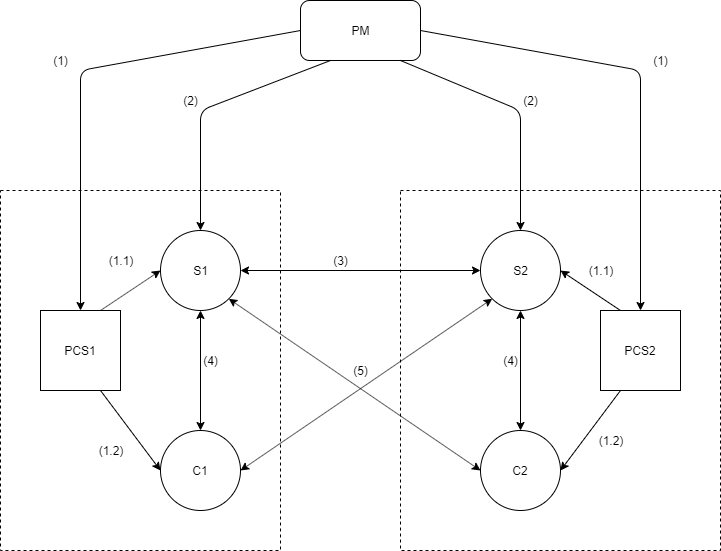
\includegraphics[width=90mm]{fault-tolerance}
\caption{System Architecture}
\label{fig:method}
\end{figure}

%-------------------------------------------------------------------------
\SubSection{Convention}

Figure 1 will be explained with the convention: “This is an example (3)”, the “(3)” in the figure corresponds to “This is an example”.

%-------------------------------------------------------------------------
\SubSection{Replication}

Whenever the PM requests the PCS to create a Server (1), PCS creates the server (1.1) and PM connects to that server (2). PM informs the server with the list of servers that already launched and also broadcasts the new server to the existing servers (2).

When a server starts, it establishes a connection with all of the servers in the list that the PM gave him, except the ones they already are connected to. The already existing servers also connect with the new server (3). At this stage, all servers have a bidirectional connection with each other (3). 

Whenever the PM requests the PCS to create a client (1), the PCS creates the client (1.2).
When a client starts, it establishes a connection with the corresponding server, that server also connects to the client (4) and broadcasts to all server replicas the new client (3). Each server replica connects to the new client and the new client also connects to each server replica that connected to him (5). At this stage, all servers have established a bidirectional connection with each server replica (3) and with each client in the system (5).

%-------------------------------------------------------------------------
\SubSection{Fault Tolerance}

Every time a client performs an action (create, join, list or close meeting), it tries to contact the original server that it's connected to (4), if that server is down, the client catches a timeout exception and tires to perform the operation with the next replica until it succeeds (5). This timeout exception will only occur the first time the client contacts the crashed server, because after the replica performs the operation correctly, the client will make new calls to the replica instead of the crashed server.
Whenever a server operates in a meeting or accepts a new client it informs all the other servers of the new information (3), and it also informs all the clients in the system (4), (5).

%-------------------------------------------------------------------------
\Section{Diffusion Algorithm}

We didn't implement a good algorithm for distributing the load of the dissemination of the meetings among the clients. In our approach, when a server changes its state, it informs all the other servers and clients in the system directly. We considered improving this algorithm by having the server inform only the other servers and clients connected to it (the server would not connect to clients connected to other servers), then each server would inform the clients connected to it. It is a better approach for scalability, but we were unable to implement this in time.

%-------------------------------------------------------------------------
\Section{Performance Evaluation}

One measure that we take to increase performance and was already mentioned in subsection (4.3), is that when a client performs the operation through a replica, the next calls he makes to the system, will be performed from that replica instead of the crashed server.

We gave priority to availability instead of performance, one of the reasons is that we didn't change the timeout of the client-server connection. If we had reduced this timeout, the system would have had more performance in recovering from faults, but the trade-off is that if the system for some reason is slow (client with low bandwidth), it could think that the server had crashed and redirect the client to another replica unnecessarily.

And as mentioned in section 5, our diffusion algorithm does not scale well.

%------------------------------------------------------------------------- 
\Section{Conclusions}

Apart from not being able to implement a better diffusion algorithm, we consider that we have addressed most goals of this project.
We implemented a robust fault tolerant system capable of performing all the client and puppet master functionalities.

\end{document}

